
\chapter{基于改进的RetianNet骨髓血细胞检测网络}
\section{引言}

第三章中,我们对比了多个单阶段与双阶段检测网络在骨髓血细胞数据上的性能,综合考虑计算量,参数量与检测精度等因素,
我们选择将性能优异的RetinaNet作为基线模型。此外我们确定了先检测再识别的骨髓血细胞处理流程,即检测网络只需要进行
对血细胞进行前景检测与坐标回归。在RetianNet基线模型中,尽管模型的检测精度已经很高,但仍然存在着漏检、密集与重叠的血细胞区域
边界检测错误等问题,如图~\ref{fig:detect_problem}所示。

骨髓血细胞检测主要有如下三个难点:(1)相比外周血红细胞、白细胞、血小板三类血细胞检测,骨髓血细胞种类繁多、
形态丰富,尺寸大小不一。(2)在骨髓涂片制作过程中,由于染色剂与光照条件的变化,多个批次的数据存在着色彩差异。此外图像
背景复杂,存在较多成熟红细胞的干扰。(3)对于骨髓细胞增生活跃的切片,存在大量血细胞密集堆叠,边缘黏连,易导致漏检、错检等问题。
因此精准检测到骨髓血细胞是一项十分具有挑战性的课题。

针对上述难点与基线模型中存在的问题,本章提出了一种改进RetinaNet网络。该方法中,我们提出了一种基于全局注意力的自底向上的路径聚合网络结构,
缩短了底层与顶层特征之间的信息传递路径,提升网络对位置特征的提取能力。此外探究了不同标签分配策略对检测性能的影响,
提出基于最优输运的标签策略用于密集区域的血细胞的标签分配,避免了模糊分配样本的出现,提高网络对血细胞的召回能力。
% 最后我们比较了空洞卷积、深度可分离卷积、可变形卷积等卷积网络,以期实现速度与检测精度的更优平衡。
在骨髓血细胞数据集上的实验结果表明,本文提出的改进方法在检测准确率上有较大的提升,达到了较为先进的性能。

\begin{figure}[htbp]                     
  \centering                      
  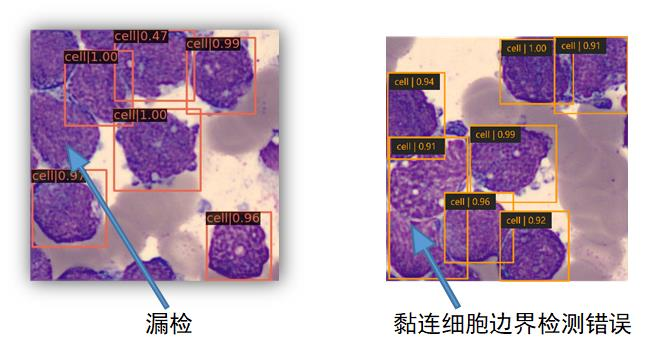
\includegraphics[width=0.65\linewidth]{detect_problem.jpg}                      
  \caption{RetinaNet基线模型检测错误示例}                      
  \label{fig:detect_problem}       
\end{figure}  

\section{改进的RetinaNet骨髓血细胞检测网络}
本章提出的改进RetinaNet网络结构如图~\ref{fig:improved_retinanet}所示,整体网络结构基于第三章的RetinaNet基线模型进行改进。骨干网络为
ResNet50用于图像特征提取,特征金字塔结构用于多尺度特征提取。锚框的尺寸、数量与分类回归网络结果与基线模型相同。
为了提高网络检测的精度,我们在特征金字塔后引入了自底向上的路径聚合模块,该模块基于全局注意力将更浅层的特征与FPN深层的进行融合,
提升网络定位特征的表达能力,此外我们引入了可变形卷积、空洞卷积等卷积模块。在训练过程中,我们使用基于最优输运的策略进行标签分配。
下面各个小节将详细介绍我们的改进点。
\begin{figure}[htbp]                     
  \centering                      
  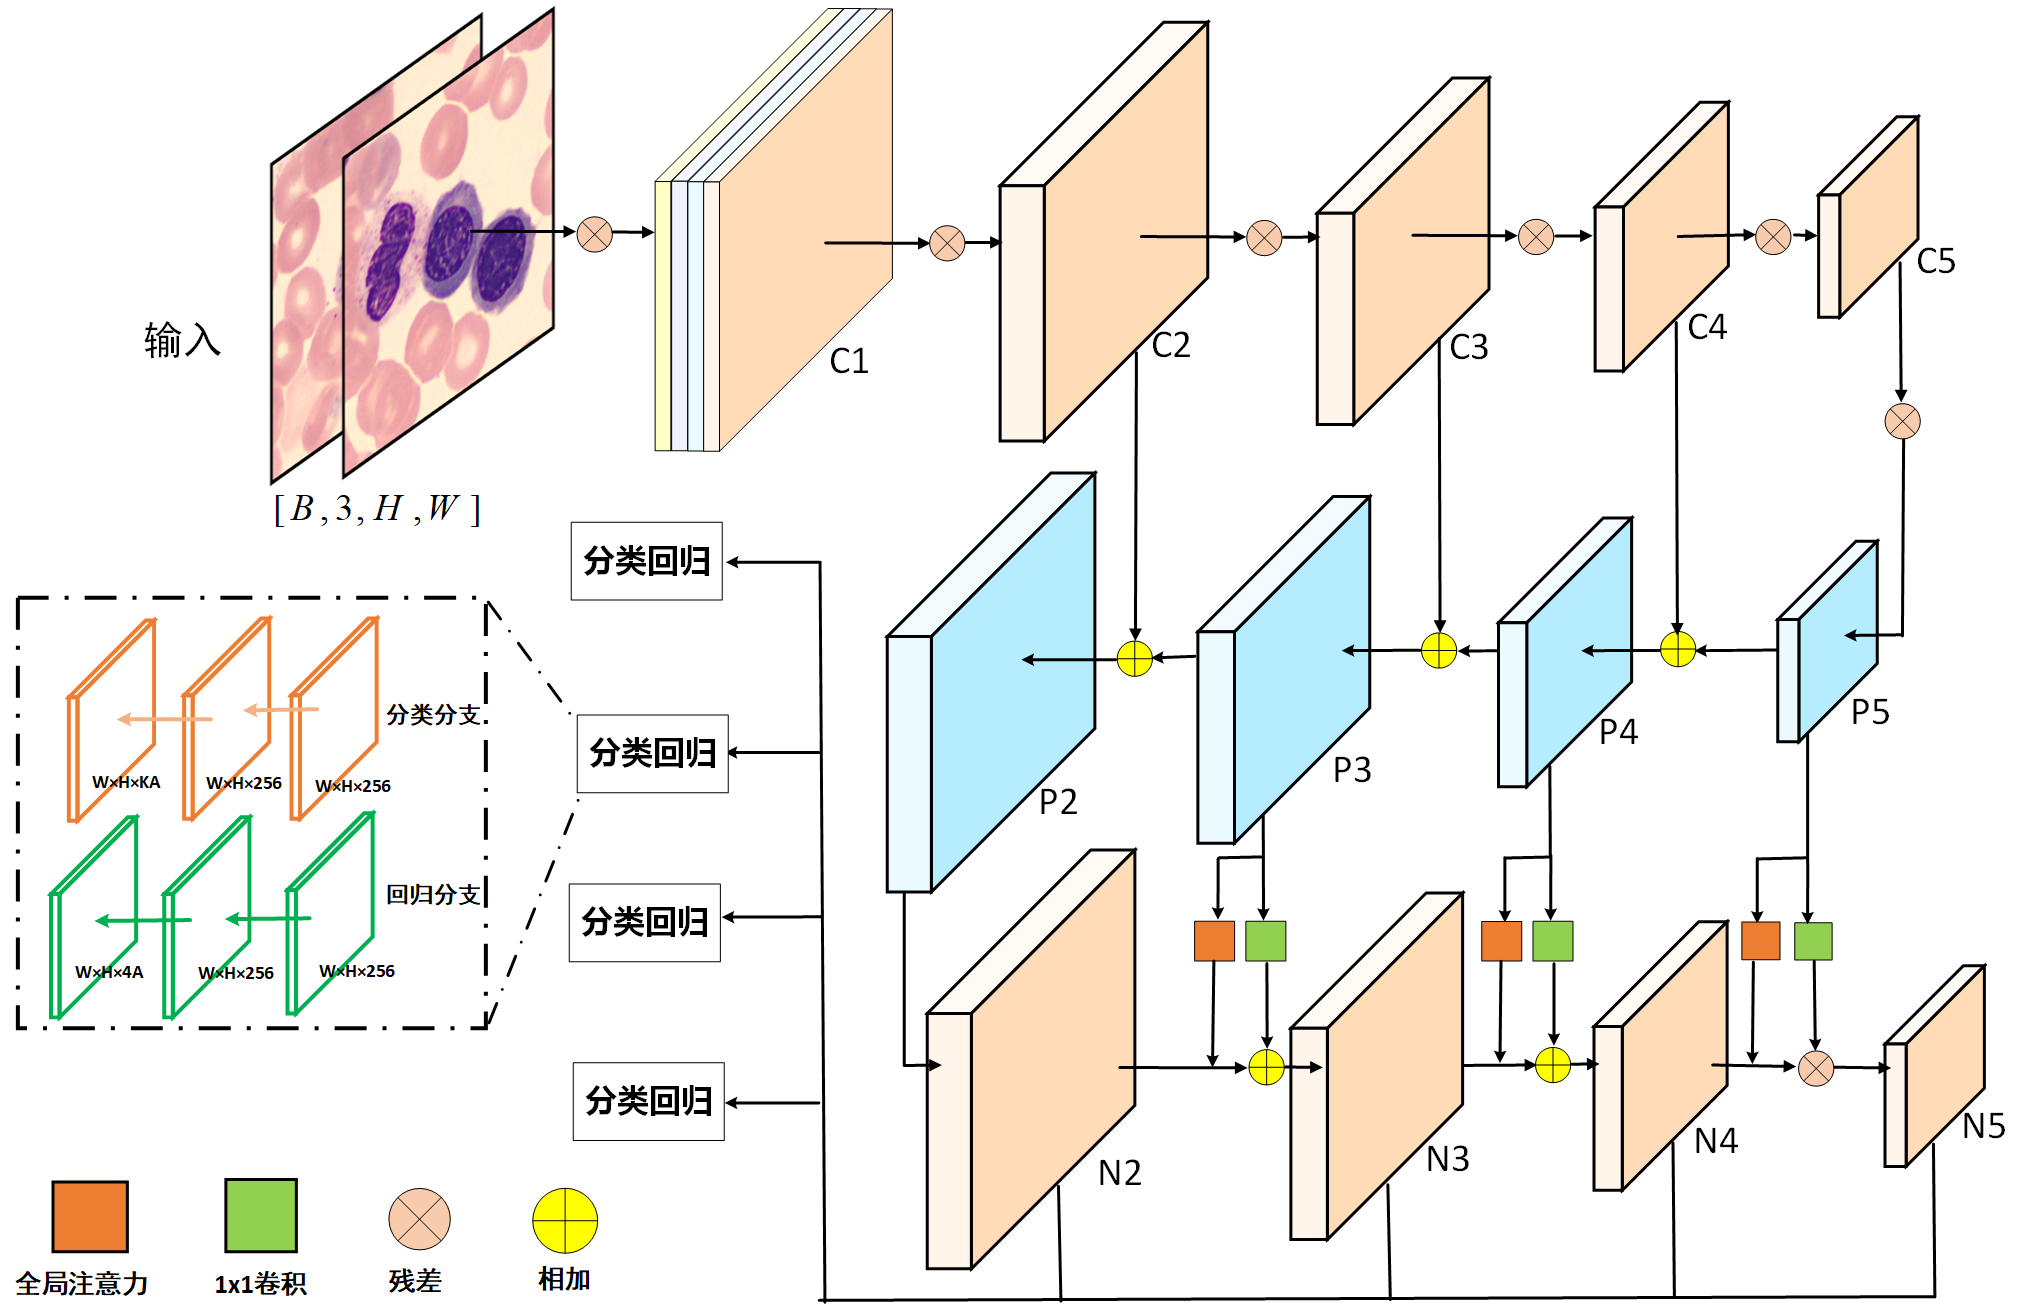
\includegraphics[width=0.95\linewidth]{improved_retinanet.png}                      
  \caption{改进的RetinaNet网络结构示意图}                      
  \label{fig:improved_retinanet}       
\end{figure}  

\subsection{基于全局注意的路径聚合网络}
ResNet50骨干网络提取了不同层级与尺度的特征图,高层次的特征图表达目标的抽象语义信息,低层次的特征图表达局部的纹理与模式信息,因此引入了
特征金字塔网络,增加自上而下的路径来传播语义强的特征,从而增强所有层次特征的分类能力。在骨髓血细胞检测任务中,我们更加关注网络对于血细胞的
定位的准确性,这些定位信息主要存在浅层特征图的边缘、纹理信息中。我们构建了自底向上的路径聚合网络,将浅层的特征与特征金字塔深层的特征图
进行融合,通过特征直连缩短了底层到顶层特征之间的信息传递路径。原始结构中底层到顶层需要需要约50层网络,如图~\ref{fig:panet}红线所示。自下而上的路径聚合网络引入了
特征直连,从底层到顶层的路径只有不到10层,如图~\ref{fig:panet}绿线所示,该路径使得浅层的纹理等高分辨定位信息可以更有效的传递到顶层,
提升网络定位特征的表达能力。
\begin{figure}[htbp]                     
  \centering                      
  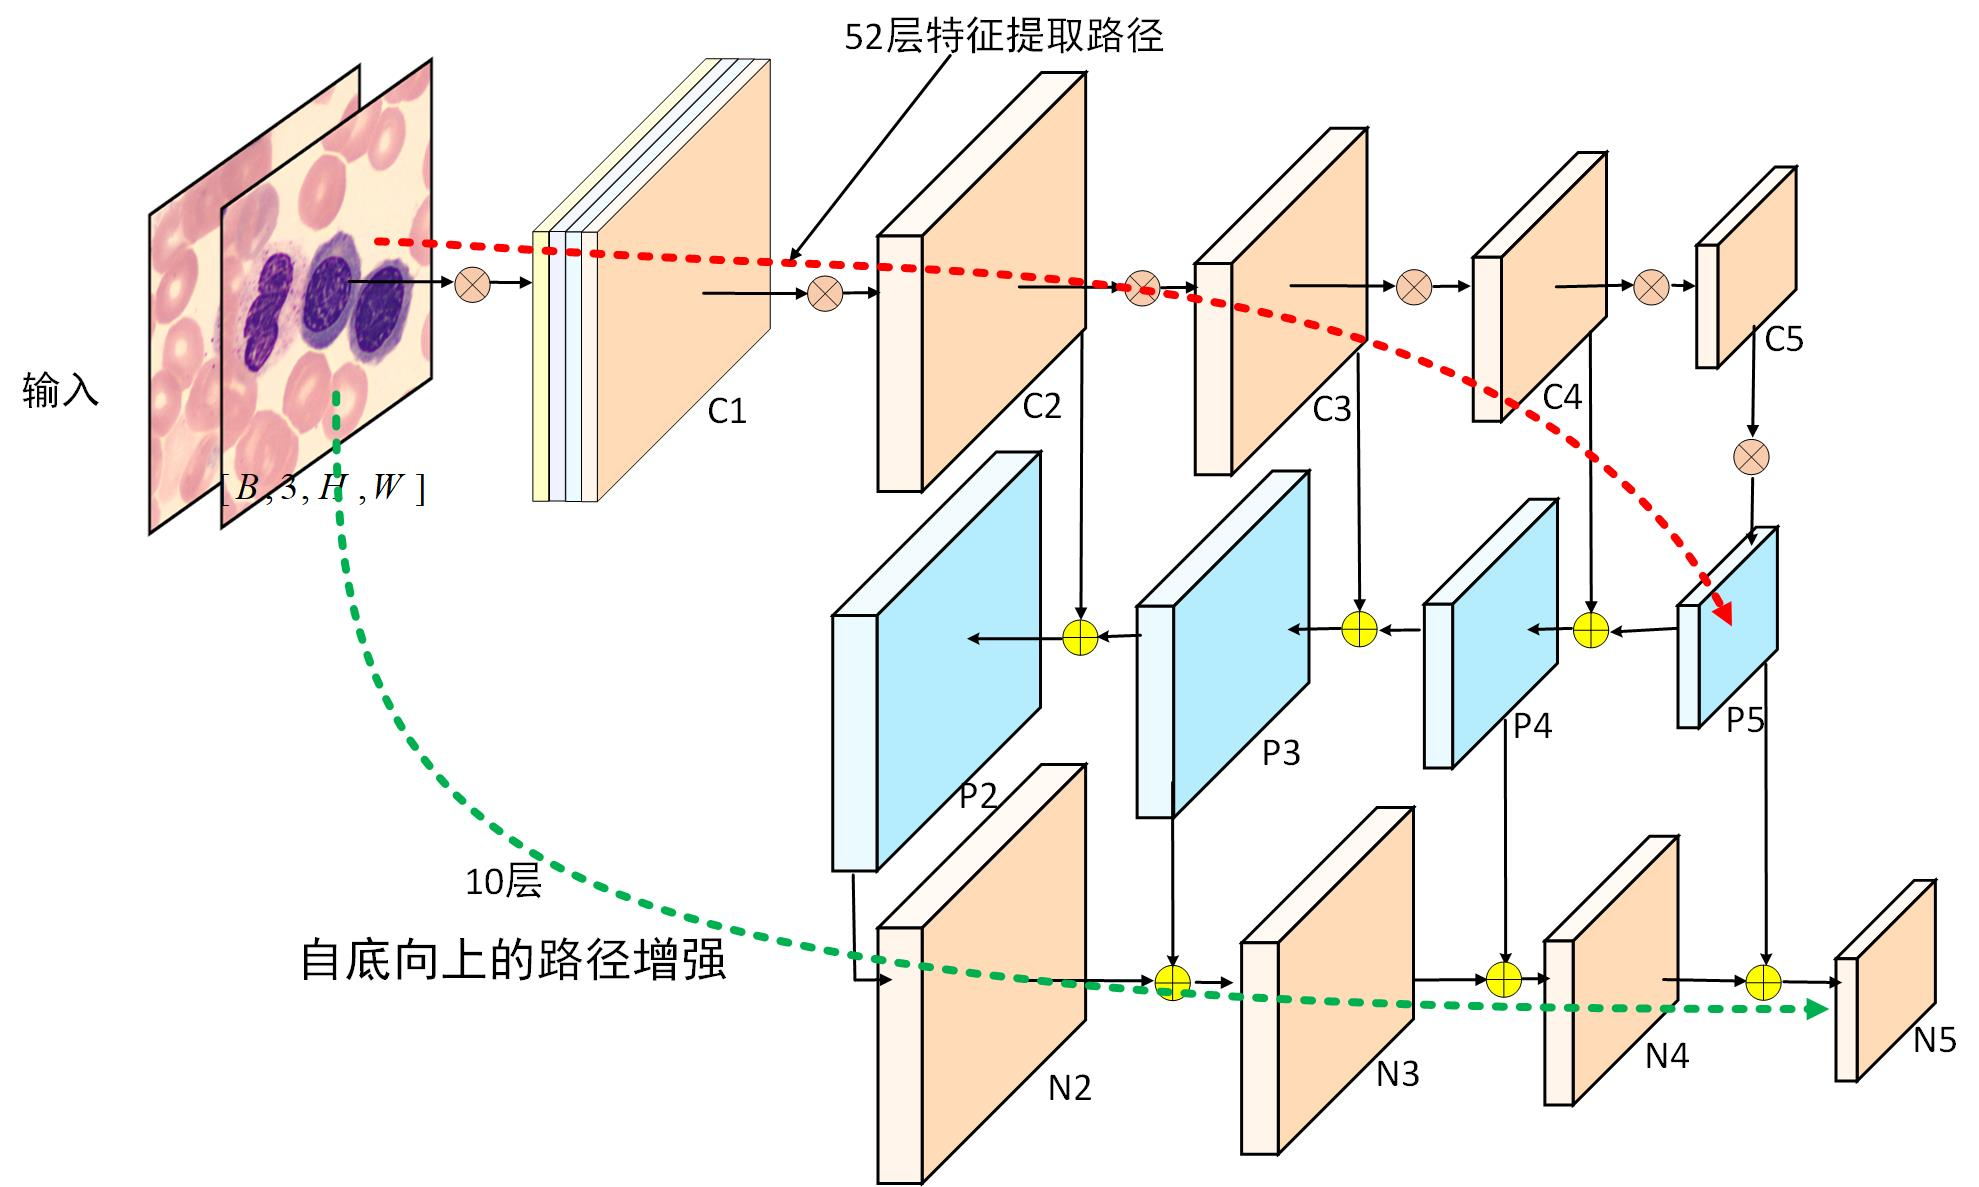
\includegraphics[width=0.75\linewidth]{panet.jpg}                      
  \caption{路径聚合网络结构示意图}                      
  \label{fig:panet}       
\end{figure}  

图中${C_2, C_3, C_4, C_5}$为ResNet50骨干网络不同阶段生成的特征图,${P_2, P_3, P_4, P_5}$为特征金字塔生成的不同级别的特征图。
自底向上的路径聚合网络从最底层的P2特征图开始,通过步长为2的卷积进行下采样并与高层的特征融合后生成新的特征图${N_2, N_3, N_4, N_5}$。
路径构建模块中使用了全局通道注意力机制,使用全局上下文信息的高层次特征指导浅层特征的筛选,该结构如图~\ref{fig:gau}所示。

\begin{figure}[htbp]                     
  \centering                      
  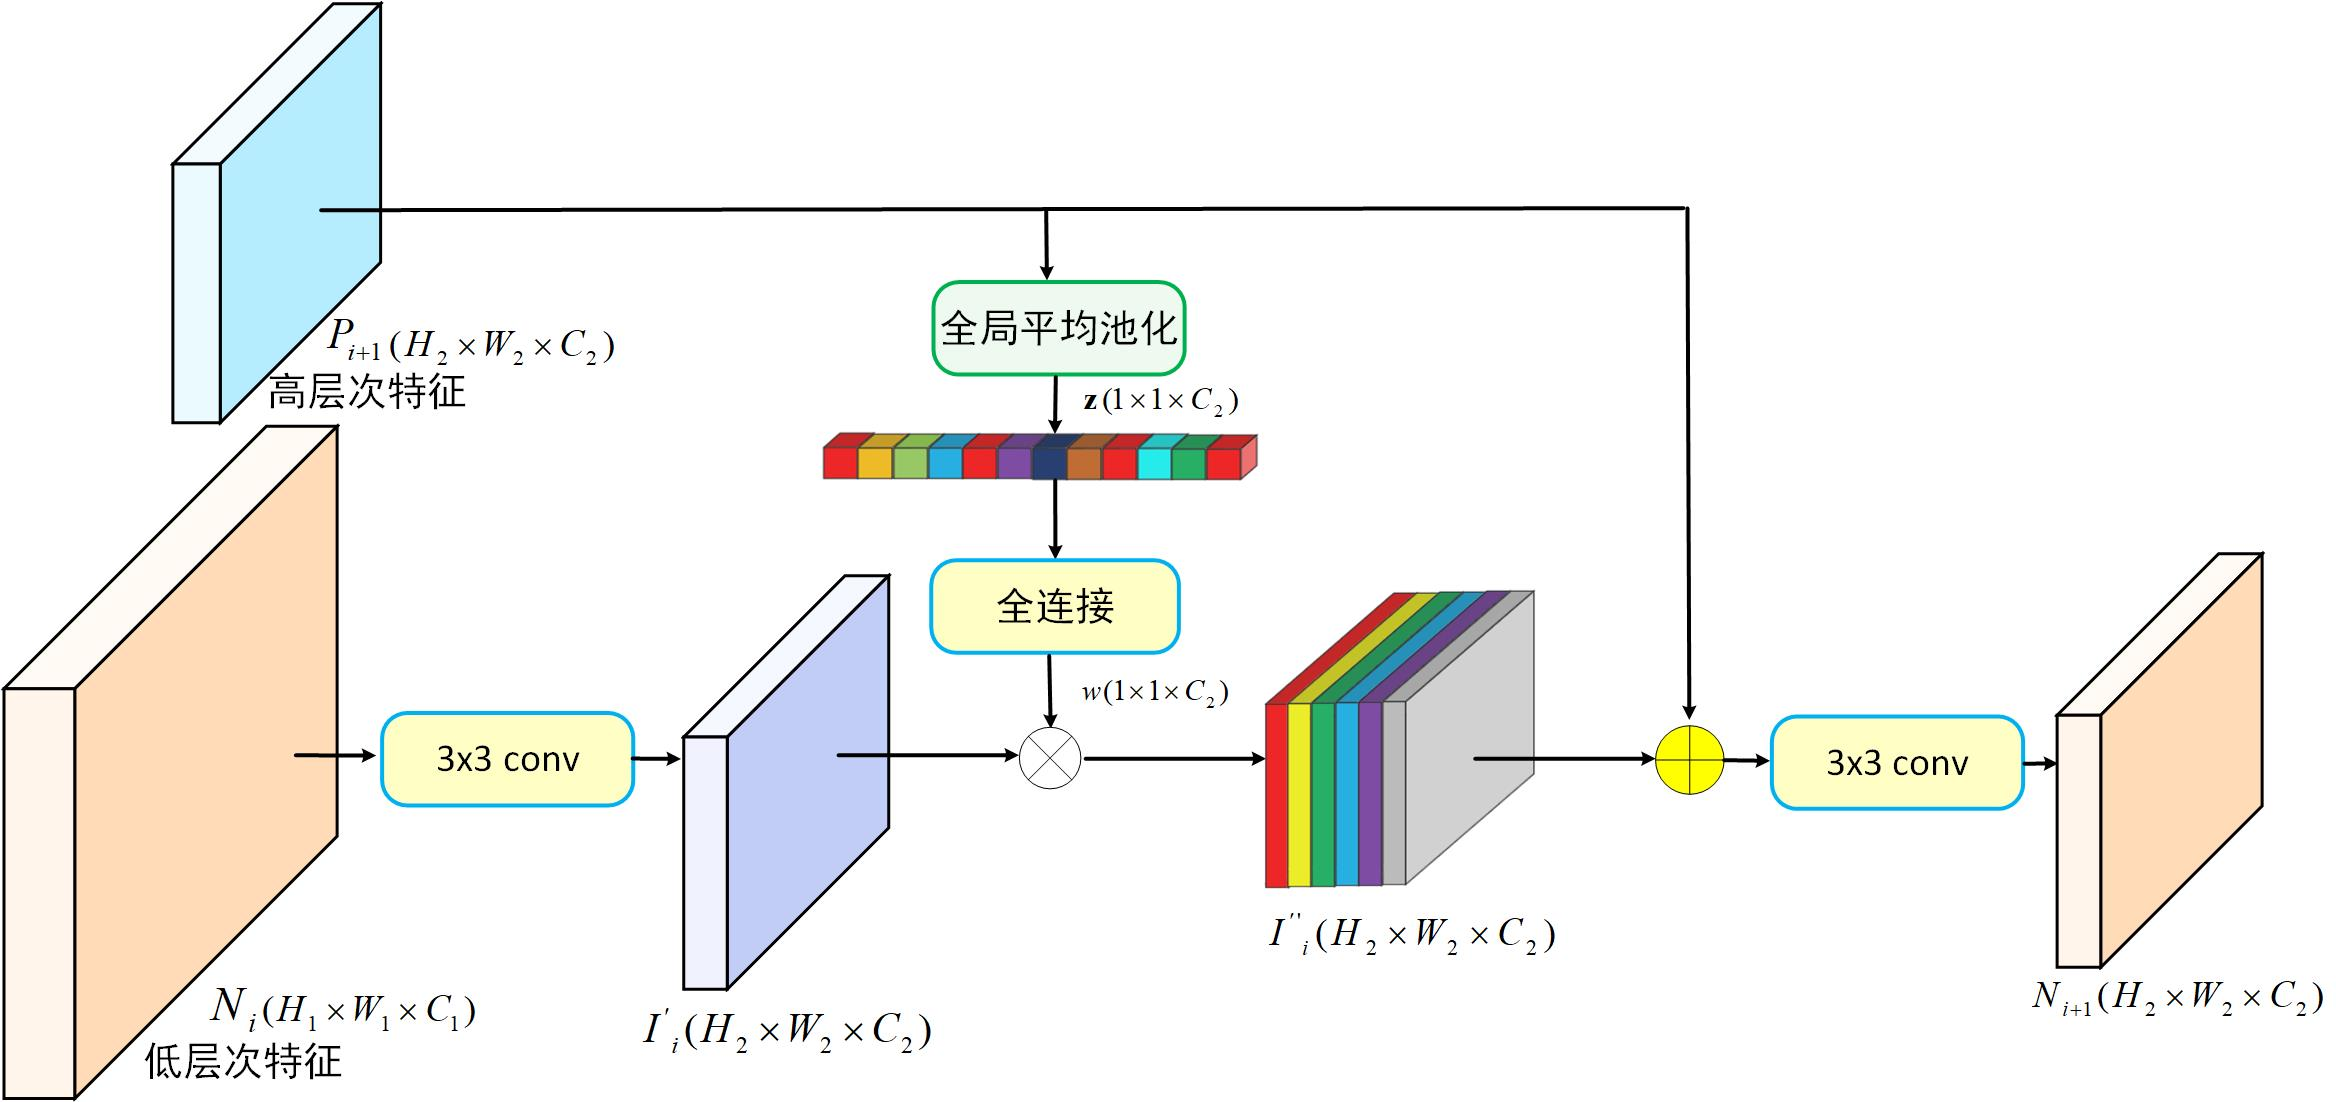
\includegraphics[width=0.95\linewidth]{gau.jpg}                      
  \caption{全局注意力模块}                      
  \label{fig:gau}       
\end{figure}  

全局注意力模块的输入分别是路径聚合网络的低层级的特征图$N_i(H_1 \times W_1 \times C_1)$与特征金字塔的高层级特征图
$P_{i + 1}(H_2 \times W_2 \times C_2)$,输出新的特征图$N_{i + 1}$。首先对特征图$N_i$经过$3\times 3$、步长为2
的卷积层降低特征图的尺寸得到$I^{\prime}_i({H_2} \times {W_2} \times {C_2})$。对高层级的特征图$P_{i + 1}$进行全局
平均池化,每个通道压缩为一个值得到C维向量$z(1 \times 1 \times {C_2})$,如式~\ref{eq:squeeze}所示:
\begin{equation}   
  \mathbf{z} = {{\bf{F}}_{sq}}\left( {{{\bf{P}}_{i + 1}}} \right) = \frac{1}{{H \times W}}\sum\limits_{i = 1}^H {\sum\limits_{j = 1}^W {{{\bf{P}}_{i + 1}}} } (i,j)
  \label{eq:squeeze} 
\end{equation}

然后使用两层全连接结构来全局建模通道之间的依赖关系,第一层全连接的输出使用ReLU激活函数,第二层使用Sigmoid激活函数,得到权重
$\mathbf{w}(1 \times 1 \times {C_2})$,如式~\ref{eq:excitation}所示。
\begin{equation}   
  {\bf{w}} = {{\bf{F}}_{ex}}({\bf{z}},{\bf{W}}) = \sigma (g({\bf{z}},{\bf{W}})) = \sigma \left( {{{\bf{W}}_2}\delta \left( {{{\bf{W}}_1}{\bf{z}}} \right)} \right)
  \label{eq:excitation} 
\end{equation}

将权重向量$\mathbf{w}$与和特征$I^{\prime}_i({H_2} \times {W_2} \times {C_2})$按通道点乘得到加权后的特征$I^{\prime \prime}_i({H_2} \times {W_2} \times {C_2})$,
如式~\ref{eq:scale}所示。
\begin{equation}   
  {\bf{I}}_i^{\prime \prime } = {{\bf{F}}_{{\rm{scale }}}}\left( {{\bf{I}}_i^\prime ,{\bf{w}}} \right) = {w_c}I^\prime_{ic}
  \label{eq:scale} 
\end{equation}

将$\bf{I}_i^{\prime \prime}$与$P_{i + 1}$逐元素相加后再经过一个$3\times3$卷积层后得到路径聚合网络的下一层特征图$N_{i + 1}$。
不断迭代上述过程,直到生成$N_5$特征图为止。最终在融合后新的特征图$N_2, N_3, N_4, N_5$上进行区域提取与坐标回归。
anchor生成与分类回归结构与RetianNet相同,在第三章已进行详细解释。

% \subsection{卷积模块}

\subsection{训练标签分配策略}
  在目标检测网络训练过程中,标签分配(Label Assignment)是非常重要的一个流程。其目的是为每一个训练样本分配分类与回归的目标,然后计算其与真值之间的损失来监督训练。
  标签分配方式为网络训练提供了判别性的监督信号,决定了网络学习与收敛的方向。本节介绍了我们训练过程中采用的不同标签分配策略,根据样本标签分配的正负权重设计,可以将
  这些方法划分为硬标签分配方法与软标签分配方法。

\subsubsection{硬标签分配策略}
硬标签分配策略假设每个锚框非正即负,若$w_{pos}, w_{neg}$分别表示样本属于正负样本的权重,则硬标签划分可以表示为
$w_{\text {pos }}, w_{n e g} \in\{0,1\}$且$w_{\text {pos }} +  w_{n e g} = 1$。这类方法的核心思想是找到一个最优划分
边界,将锚框分割为正样本集合与负样本集合。

RetinaNet与Faster-RCNN网络采用的是最常用的基于交并比最大化的标签分配策略(MaxIouAssigner)。
该方法主要由以下的六个步骤:(1)初始化,将正样本集合$P$、负样本集合$N$设置为空集,将所有锚框设置为忽略样本;
(2)计算多尺度特征图上所有锚框与所有真实框之间的交并比

\subsubsection{软标签分配策略}

\section{算法实现与实验结果分析}
\subsection{实验环境}
\subsubsection{数据集介绍}

骨髓血细胞图像来自邃蓝智能科技(上海)有限公司合作医院提供,首先采用第2.1小节阐述的主动学习标注策略进行边界框的标注。
我们总共标记了6821张血细胞图像,训练集与测试集按照4:1的比例进行随机划分,训练集包含了5456张图像,测试集包含了1365张图像。
通常每个图像中包含1到10个有核血细胞,数据集总共标记了11352个血细胞,训练集有9065个血细胞,测试集有2287个血细胞。数据集的分布如
表~\ref{table:cell_detect1}所示:

\begin{table}
  \caption{骨髓血细胞检测数据集分布}   
  \centering 
  \label{table:cell_detect1}
  \begin{tabular}{ccccc}
    \toprule[2pt]
    序号 & 类别名  &  类别简写 & 训练集数量 & 测试集数量 \\
    \midrule[1.5pt] 
    1 & 原始细胞 & Prim & 1856 & 467 \\ 
    2 & 淋巴细胞 & Lym & 996 & 226   \\ 
    3 & 单核细胞 & Mono & 206 & 52   \\ 
    4 & 浆细胞 & Plas & 272 & 70   \\ 
    5 & 红细胞 & Red & 1880 & 503   \\ 
    6 & 早幼粒细胞 & Promy & 357 & 107   \\ 
    7 & 嗜中性中幼粒细胞 & Myelo & 701 & 150   \\ 
    8 & 嗜中性晚幼粒细胞 & Late & 503 & 144   \\ 
    9 & 嗜中性杆状核细胞 & Rods & 998 & 241   \\  
    10 & 嗜中分叶核细胞 & Lobu & 821 & 195   \\  
    11 & 嗜酸性粒细胞 & Eosl & 475 & 132   \\  
    \hline
    总计 &   &   & 9065 & 2287 \\
    \bottomrule[2pt]      
  \end{tabular} 
\end{table}


\subsection{实验结果与分析}
\subsubsection{评价指标} 
\subsubsection{实验结果}
\subsubsection{路径聚合网络}
\subsubsection{标签分配策略}
\subsubsection{不同卷积模块对实验结果影响}
\section{小结}


